\documentclass[xcolor=dvipsnames,table]{beamer}
\useinnertheme{rounded}
\useoutertheme{infolines}

\usepackage[portuguese]{babel}
\usepackage[utf8]{inputenc}
\usepackage{url}
\usepackage{multicol}
\usepackage{multirow}

\title{Pesquisas em MDS e CEPH}
\subtitle{Tópicos em Redes de Computadores (INFO-7065)}
\author{Josiney de Souza (josiney.souza@ifc.edu.br)}
\institute{UFPR / DInf}
\date{\today}

%%% Apagar barra de navegacao:
% https://stackoverflow.com/questions/3210205/how-to-get-rid-of-navigation-bars-in-beamer
% https://stackoverflow.com/questions/1435837/how-to-remove-footers-of-latex-beamer-templates
\beamertemplatenavigationsymbolsempty
%%% Remover o titulo, autor e data do rodape:
% https://tex.stackexchange.com/questions/113443/remove-author-and-institution-in-footline
\beamertemplatefootempty

%%% Cores das fontes:
% https://en.wikibooks.org/wiki/LaTeX/Colors
\definecolor{ifvermelho}{RGB}{200,12,15}
\definecolor{ifverde}{HTML}{2F9E41}
% Mais cores feitas com http://coolors.co
\definecolor{ifvermelho2}{HTML}{B60B0E} % Nome: International Orange Engineering
\definecolor{ifvermelho3}{HTML}{A50A0D} % Nome: Rufous
\definecolor{ifmeioesq}{HTML}{A2311C} % Nome: Chinese Red
\definecolor{ifmeio}{HTML}{7C5528} % Nome: Coyote Brown
\definecolor{ifmeiodir}{HTML}{567A35} % Nome: Sap Green
\definecolor{ifverde2}{HTML}{42A752} % Nome: Green Pigment
\definecolor{ifverde3}{HTML}{53AF62} % Nome: Medium Sea Green

% https://tex.stackexchange.com/questions/133820/beamer-how-to-change-color-of-infolines-and-frame-title
\setbeamercolor{title}{fg=Red}
\setbeamercolor{frametitle}{fg=Red}
\setbeamercolor{section in head/foot}{fg=White,bg=ifvermelho}
\setbeamercolor{subsection in head/foot}{fg=ifverde}

%%% Cores das caixas de block, exemplo e alerta
% https://tex.stackexchange.com/questions/33231/how-to-change-the-color-of-a-block-within-a-custom-beamer-sty-theme-file
\setbeamercolor{block title}{fg=White,bg=ifverde2}
\setbeamercolor{block body}{fg=White,bg=ifverde3}
% https://tex.stackexchange.com/questions/73163/change-color-scheme-for-example-box-in-beamer
\setbeamercolor{block title example}{fg=White,bg=ifmeio}
\setbeamercolor{block body example}{fg=White,bg=ifmeiodir}
% https://tex.stackexchange.com/questions/96686/change-color-of-itemize-in-beamer-alertblock
\setbeamercolor{block title alerted}{fg=White,bg=ifvermelho3}
\setbeamercolor{block body alerted}{fg=White,bg=ifvermelho2}

%%% Mostrar o sumario novamente antes do inicio da proxima secao
% https://pt.overleaf.com/learn/latex/beamer
\AtBeginSection[]
{\small
  \begin{frame}[plain]
    \frametitle{Sumário}
%    \tableofcontents[currentsection]
	\begin{multicols}{2}
	\tableofcontents[currentsection]
	\end{multicols}
  \end{frame}
}

%%% Plano de fundo usado no modelo ODT/DOC/DOCX da Cecom
\usebackgroundtemplate%
{%
    
\includegraphics[width=\paperwidth,height=\paperheight]{fundo.jpg}%
}



%%%%%%%%%%%%%%%%%%%%%%%%%%%%%%%%%%%%%%%%%%%%%%%%%%%
%%%%%%%%%%%%%%% Início do documento %%%%%%%%%%%%%%%
%%%%%%%%%%%%%%%%%%%%%%%%%%%%%%%%%%%%%%%%%%%%%%%%%%%
\begin{document}

%%%%% Primeira página do modelo abaixo - PODE SER REMOVIDA, SE DESEJAR %%%%%
%%% Centralizando o titulo da primeira pagina
% https://stackoverflow.com/questions/2365539/centering-titles-when-using-the-beamer-class-in-latex
%%% Removendo as formatacoes do slide
% https://tex.stackexchange.com/questions/281334/left-aligned-title-page-in-beamer-boadilla-usetheme
%{
%\usebackgroundtemplate%
%{%
%    
\includegraphics[width=\paperwidth,height=\paperheight]{primeira-pag-menor.jpg}%
%}
%\begin{frame}[plain]{\centerline{\inserttitle}}
%\end{frame}
%}
%%%%% Primeira página do modelo acima - PODE SER REMOVIDA, SE DESEJAR %%%%%

\begin{frame}[plain]{}
    \maketitle
\end{frame}

{\small
\begin{frame}[plain]{Sumário}
%    \tableofcontents
	\begin{multicols}{2}
	\tableofcontents
	\end{multicols}
\end{frame}
}

%%%%%%%%%%%%%%%%%%%%%%%%%%%%%%%%%%%%%%%%%%%%%%%%%%%%%%%%%%%%%%%%%%%%%
\section{Introdução}
\subsection{Sistemas de Arquivos}
\begin{frame}{Visão geral de sistemas de arquivos}
	\begin{itemize}
		\item Computadores usam Sistemas Operacionais (SO's)
		\item Em nível físico, SO's estão em memória (RAM, HD, \textit{flash}, SSD, memória persistente)
		\item Em nível lógico, SO's usam sistemas de arquivos (\textit{file systems} - FS)
		\item Podem ser locais ...
		\begin{itemize}
			\item EXT4
			\item XFS
			\item NTFS
		\end{itemize} \pause
		\item ou remotos:
		\begin{itemize}
			\item NFS
			\item CEPH
			\item EOS
			\item GlusterFS
			\item Lustre
		\end{itemize}
	\end{itemize}
\end{frame}

%\begin{frame}{}
%	T
%\end{frame}

%%%%%%%%%%%%%%%%%%%%%%%%%%%%%%%%%%%%%%%%%%%%%%%%%%%%%%%%%%%%%%%%%%%%%
\section{Sistemas Distribuídos}
\subsection{Revisão}
\begin{frame}{Sistemas distribuídos}
	Sobre a arquitetura e organização:
	\begin{description}
		\item[Centralizado] clientes e servidores;
		\item[Descentralizado] P2P (pode ser cliente e servidor ao mesmo tempo);
		\item[Híbrido] P2P com componentes centralizados.
	\end{description}
	
	\pause

	Sobre o modelo temporal:
	\begin{description}
		\item[assíncrono] não se fala em tempo;
		\item[parcialmente síncrono] entre assíncrono e síncrono. Algumas asserções podem ser feitas;
		\item[síncrono] sabe-se o tempo máximo para transmissão de mensagem e execução de tarefas.
	\end{description}
\end{frame}

\subsection{Modelo de Falhas}
\begin{frame}{Sistemas distribuídos}
	Sobre o modelo de falhas:
	\begin{description}
		\item[Crash] cessa a computação e para de responder
		\item[Omissão] falha em responder (não processa o resultado ou não o trata)
		\item[Bizantino] age diferente do normal ou esperado (podem ser nodos maliciosos)
	\end{description}
	
	\pause
	
	Sobre o número de nodos para um limiar ``f'' de falhas:
	\begin{center}
		\begin{tabular}{||c|c||}
			\hline
			\textbf{Tipo de falha} & \textbf{Número de nodos} \\
			\hline
			\hline
			Crash & 2f + 1 \\
			\hline
			Bizantina & 3f + 1 \\
			\hline
		\end{tabular}
	\end{center}
\end{frame}

\subsection{Consenso}
\begin{frame}{O consenso}
	O consenso em sistemas distribuídos:
	\begin{itemize}
		\item é o problema de múltiplos nodos concordarem sobre uma sequência de valores
		\item algoritmo de consenso faz com que os nodos corretos executem o mesmo comando, na mesma ordem e cheguem ao mesmo estado
	\end{itemize} \pause

	\begin{center}
		\begin{tabular}{|c|c|c|}
			\hline
			\textbf{Modelo de falhas} & \textbf{Algoritmo de Consenso} & \textbf{Consenso de valor} \\
			\hline
			\hline
			Crash & Paxos (1989, 1998) & Único \\
				& Multi-Paxos & Geral \\
				& Cheap Paxos & Geral \\
				& Fast Paxos & Geral \\
				& Raft (2014) & Geral \\
			\hline
			Bizantino & Byzantine Paxos & Único \\
				& PBFT & Geral \\
			\hline
		\end{tabular}
	\end{center}
\end{frame}

%\begin{frame}{}
%	T
%\end{frame}

%%%%%%%%%%%%%%%%%%%%%%%%%%%%%%%%%%%%%%%%%%%%%%%%%%%%%%%%%%%%%%%%%%%%%
\section{MDS}
\subsection{Visão Geral}
\begin{frame}{Por que metadados?}
	Por que se pensaria em metadados?
	\begin{itemize}
		\item \textit{Big data} e \textit{cloud} estão em alta
		\item Escala de TiB, PiB, EiB
		\item Aplicações demandam armazenamento
		\item É necessário gerenciar os dados e seus metadados
	\end{itemize}
\end{frame}

\begin{frame}{Os metadados}
	Em sistemas de arquivos, em relação aos metadados:
	\begin{itemize}
		\item são os dados responsáveis por manter o \textit{namespace}, semântica de permissões e localização dos dados dos arquivos;
		\item operações com eles podem representar até 80\% das operações totais;
		\item representam apenas 1\% do dado em si;
		\item informações sobre tipo, tamanho, estado;
		\item informações sobre permissões, propriedade, tempos;
		\item informações sobre os blocos dos dados em si.
	\end{itemize}
\end{frame}

\begin{frame}{Os metadados}
	\begin{center}
		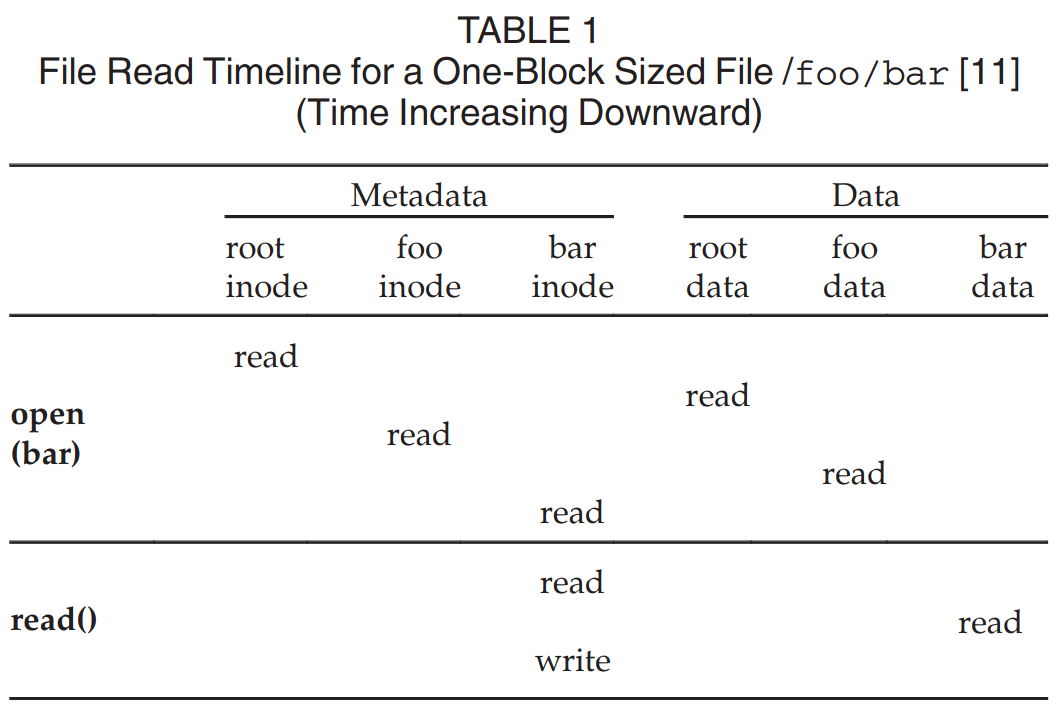
\includegraphics[scale=0.25]{metadados1.png}
	\end{center}
	Fonte: [Dai et al., 2022]
\end{frame}

\subsection{Workloads}
\begin{frame}{Os metadados: cargas de trabalho}
	Estudos observaram o seguinte sobre a carga de trabalho dos sistemas:
	\begin{itemize}
		\item para o refinamento de resultados, mais de 95\% das buscas são para vários atributos de metadados
		\item 33\% das buscas são limitadas para uma área relacionada do \textit{namespace}
		\item quase 25\% das buscas que os usuários pensam ser importantes são para várias versões do metadado

		\pause

		\item a maioria dos valores dos atributos estão sob localidade espacial (ex.: /home/jsouza)
		\item há um grau de assimetria alto e valores predominantes ocupam mais do espaço de valor (ex.: 80\% dos arquivos têm mais valores em comum que os outros 20\% para os atributos \texttt{ext} e \texttt{size})
	\end{itemize}
\end{frame}

\begin{frame}{Os metadados: cargas de trabalho}
	Estudos observaram o seguinte sobre a carga de trabalho dos sistemas:
	\begin{itemize}
		\item de 60 sistemas de arquivos, 90\% dos diretórios têm menos que 128 entradas de diretórios
		\item diretórios grandes continuam a crescer com o aumento da capacidade do armazenamento
		\item 64\% das mídias têm menos que 64 KiB
		\item 90\% das árvores de diretórios não passam de profundidade 16
		\item na manipulação, geralmente se executa \texttt{open} e/ou \texttt{readdir}
	\end{itemize}
\end{frame}

\subsection{Arquiteturas}
\begin{frame}{Os metadados: arquiteturas}
	Acerca de um MDS (\underline{M}eta\underline{D}ata \underline{S}erver), as arquiteturas de gerenciamento utilizadas para os metadados são:
	\begin{itemize}
		\item Sem MDS, no mesmo servidor dos dados
		\item Com um MDS único
		\item Com um MDS distribuído
%		\begin{itemize}
	\end{itemize}
\end{frame}

\begin{frame}{Os metadados: arquiteturas}
	\begin{center}
		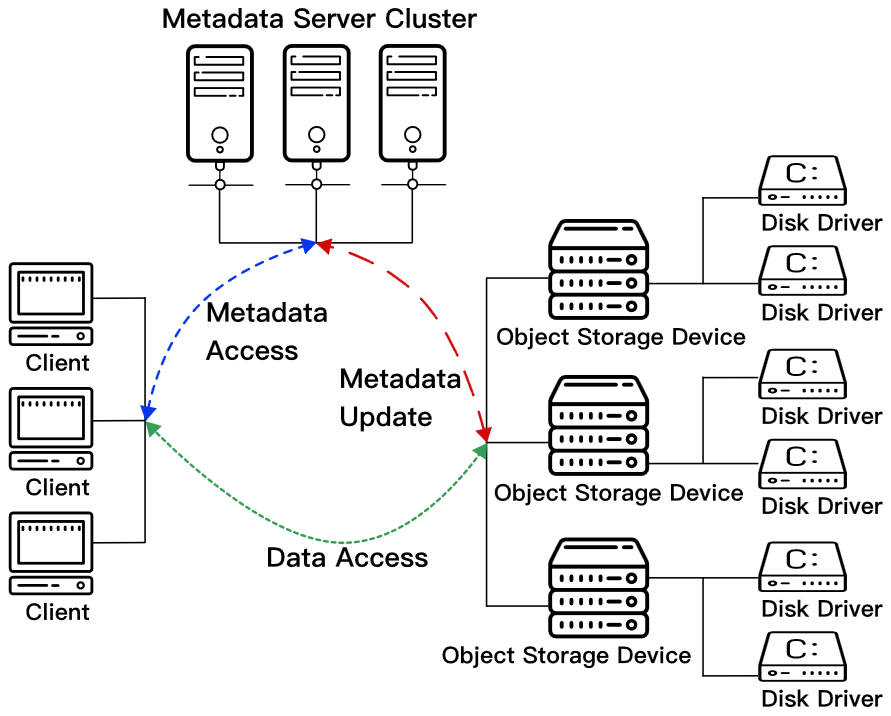
\includegraphics[scale=0.25]{metadados2.png}
	\end{center}
	Fonte: [Dai et al., 2022]
\end{frame}

\subsection{Campos de Pesquisa}
\begin{frame}{Os metadados: campos de pesquisa}
	São campos de pesquisa atualmente:
	\begin{itemize}
		\item Alta escalabilidade
		\item Alto desempenho
		\item Alta disponibilidade
	\end{itemize}
\end{frame}

\subsection{Alta Escalabilidade}
\begin{frame}{Alta escalabilidade}
	É feita através da divisão de espaços.

	\begin{itemize}
		\item A divisão dos metadados podem ser sobre algumas informações
		\begin{itemize}
			\item nome do caminho
			\item tamanho da subárvore
		\end{itemize}
		\item Características:
		\begin{itemize}
			\item Localidade
			\item Balanceamento de carga
		\end{itemize}
		\item Métodos usados:
		\begin{enumerate}
			\item Estáticos
			\item Dinâmicos
		\end{enumerate}
	\end{itemize}
\end{frame}

\subsubsection{Métodos Estáticos}
\begin{frame}{Alta escalabilidade: (1) métodos estáticos}
	Modelos dos métodos \underline{estáticos}:
	\begin{itemize}
		\item \textbf{Particionamento de subárvore}
		\begin{itemize}
			\item NFS
			\item administrador decide como dividir os fragmentos
			\item aumenta a localidade
			\item não consegue lidar bem com desbalanceamento
		\end{itemize}
		\item \textbf{Mapeamento baseado em \textit{hash}}
		\begin{itemize}
			\item aplicar função de \textit{hash} sobre o arquivo
			\item descobre-se o MDS
			\item aumenta o balanceamento
			\item tende à baixa localidade
		\end{itemize}
	\end{itemize}
\end{frame}

%\begin{frame}{Alta escalabilidade: (1) métodos estáticos}
%	Modelos dos métodos \underline{estáticos}:
%	\begin{itemize}
%		\item \textbf{Particionamento de subárvore}
%		\begin{itemize}
%			\item NFS
%			\item administrador decide como dividir os fragmentos
%			\item aumenta a localidade
%			\item eficiente quando os metadados são repetidamente acessados por um número pequeno de servidores
%			\item não consegue lidar bem com desbalanceamento
%			\item gargalo para arquivos em uma mesma subárvore
%			\item replicação de subárvore pode ajudar
%			\item custo de espaço e de calcular consistência
%		\end{itemize}
%	\end{itemize}
%\end{frame}
%
%\begin{frame}{Alta escalabilidade: (1) métodos estáticos}
%	Modelos dos métodos \underline{estáticos}:
%	\begin{itemize}
%		\item \textbf{Mapeamento baseado em \textit{hash}}
%		\begin{itemize}
%			\item aplicar função de \textit{hash} sobre o arquivo
%			\item descobre-se o MDS
%			\item aumenta o balanceamento
%			\item tende à baixa localidade
%			\item mudar caminhos aumenta a carga de rede
%		\end{itemize}
%	\end{itemize}
%\end{frame}

\begin{frame}{Alta escalabilidade: (1) métodos estáticos}
	Modelos dos métodos \underline{estáticos}:
	\begin{itemize}
		\item \textbf{Híbrido (subárvore + \textit{hash})}
		\begin{itemize}
			\item teoricamente, o melhor de dois mundos
		\end{itemize}
			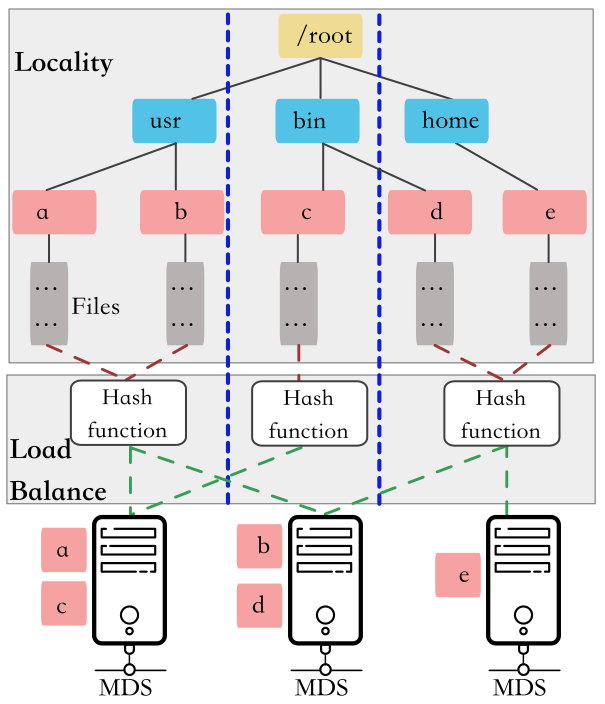
\includegraphics[scale=0.2]{esc-est-hib.png}
		\begin{itemize}
			\item mesmo assim, sobrecarga de rede na migração de metadados
		\end{itemize}
	\end{itemize}
\end{frame}

\subsubsection{Métodos Dinâmicos}
\begin{frame}{Alta escalabilidade: (2) métodos dinâmicos}
	Modelos dos métodos \underline{dinâmicos}:
	\begin{itemize}
		\item Divisão dinâmica dos espaços
		\item Na mudança da carga de trabalho, dados são rearranjados entre MDS;
		\item Modelos:
		\begin{enumerate}
			\item Subárvore
			\item Subconjunto de itens de diretório
			\item \textit{Hashing}
		\end{enumerate}
	\end{itemize}	
\end{frame}

\begin{frame}{Alta escalabilidade: (2) métodos dinâmicos}
	Modelos dos métodos \underline{dinâmicos}:
	\begin{itemize}
		\item \textbf{Subárvore}
		\begin{itemize}
			\item Migrar cargas de trabalho dos nodos sobrecarregados
			\item Decaimento de contador de tempo exponencial
			\item O \textit{load} é comparado frequentemente
			\item Sofre com migração de dados não controlada
		\end{itemize}
		\item \textbf{Subconjunto de itens de diretório}
		\begin{itemize}
			\item Cada diretório em um servidor primário aleatório
			\item Em um limiar, divide em subconjuntos em secundários aleatórios
			\item LSM-tree, LevelDB, Sorted String Table (SSTable)
			\item Depende fortemente da exploração de \textit{cache}
		\end{itemize}
		\item \textbf{\textit{Hashing}}
		\begin{itemize}
			\item Usa \textit{hash} e as posições dos bits do \textit{hash}
			\item Balanceado em armazenamento mas com problemas com \textit{hotspots}
			\item Estima a frequência de acessos de dados
			\item Existem trabalhos com \textit{Software Defined Network} (SDN)
		\end{itemize}
	\end{itemize}
\end{frame}

%\begin{frame}{Alta escalabilidade: (2) métodos dinâmicos}
%	Modelos dos métodos \underline{dinâmicos}:
%	\begin{itemize}
%		\item \textbf{Subárvore}
%		\begin{itemize}
%			\item Problema de balanceamento de carga
%			\item Migrar cargas de trabalho dos nodos sobrecarregados
%			\item CEPH
%			\item Decaimento de contador de tempo exponencial
%			\item Novos acessos aumentam o contador de tempo em todo o caminho
%			\item O \textit{load} é comparado frequentemente
%			\item Nodo responsável: caminho (\textit{path}) ou \textit{hash} do \texttt{inode}
%			\item Sofre com migração de dados não controlada
%		\end{itemize}
%	\end{itemize}
%\end{frame}
%
%\begin{frame}{Alta escalabilidade: (2) métodos dinâmicos}
%	Modelos dos métodos \underline{dinâmicos}:
%	\begin{itemize}
%		\item \textbf{Subconjunto de itens de diretório}
%		\begin{itemize}
%			\item IndexFS
%			\item Trata metadados e pequenos arquivos da mesma forma
%			\item Cada diretório em um servidor primário aleatório, junto com suas entradas
%			\item Ao chegar em um limiar, divide em subconjuntos em secundários/\textit{backups} também aleatórios
%			\item LSM-tree
%			\item LevelDB
%			\item Sorted String Table (SSTable)
%			\item Depende fortemente da exploração de \textit{cache}
%		\end{itemize}
%	\end{itemize}
%\end{frame}
%
%\begin{frame}{Alta escalabilidade: (2) métodos dinâmicos}
%	Modelos dos métodos \underline{dinâmicos}:
%	\begin{itemize}
%		\item \textbf{\textit{Hashing}}
%		\begin{itemize}
%			\item Em nível de bloco
%			\item Usa \textit{hash} e as posições dos bits do \textit{hash}
%			\item Balanceado em espaço de armazenamento mas com problemas com \textit{hotspots}
%			\item Estima a frequência de acessos de dados
%			\item Existem trabalhos com \textit{Software Defined Network} (SDN)
%		\end{itemize}
%	\end{itemize}
%\end{frame}

\begin{frame}{Alta escalabilidade: sumarização}
	Sumarizando os métodos de alta escalabilidade:
\begin{table}[]
\begin{tabular}{|l|lll|lll|}
\hline
\multirow{2}{*}{Métrica} & \multicolumn{3}{l|}{Estático}                                                 & \multicolumn{3}{l|}{Dinâmico}                                                      \\ \cline{2-7} 
                         & \multicolumn{1}{l|}{Subárvore} & \multicolumn{1}{l|}{\textit{Hash}} & Híbrido & \multicolumn{1}{l|}{Subárvore} & \multicolumn{1}{l|}{Diretório} & \textit{Hashing} \\ \hline
Hotspot                  & \multicolumn{1}{l|}{Sim}       & \multicolumn{1}{l|}{Não}           & Não     & \multicolumn{1}{l|}{Sim}       & \multicolumn{1}{l|}{Sim}       & Sim              \\ \hline
Bal. Carga                    & \multicolumn{1}{l|}{Ruim}      & \multicolumn{1}{l|}{Bom}           & Bom     & \multicolumn{1}{l|}{Bom}       & \multicolumn{1}{l|}{Bom}       & Bom              \\ \hline
Localidade               & \multicolumn{1}{l|}{Bom}       & \multicolumn{1}{l|}{Ruim}          & Bom     & \multicolumn{1}{l|}{Bom}       & \multicolumn{1}{l|}{Bom}       & Ruim             \\ \hline
Escalab.                 & \multicolumn{1}{l|}{Custa}     & \multicolumn{1}{l|}{Custa}         & Custa   & \multicolumn{1}{l|}{B. custo}  & \multicolumn{1}{l|}{Custa}     & Custa            \\ \hline
Troca nome               & \multicolumn{1}{l|}{Custa}     & \multicolumn{1}{l|}{Custa}         & Custa   & \multicolumn{1}{l|}{Custa}     & \multicolumn{1}{l|}{Custa}     & Custa            \\ \hline
\end{tabular}
\end{table}
Fonte: adaptado de [Dai et al., 2022]
\end{frame}

\subsection{Alto Desempenho}
\begin{frame}{Alto desempenho}
	Os servidores de metadados podem considerar o alto desempenho sob as seguintes óticas:
	\begin{enumerate}
		\item \textit{Cache} e replicação
		\item Recuperação de metadados
		\item Metadados de valor agregado
	\end{enumerate}
\end{frame}

\subsubsection{\textit{Cache} e Replicação}
\begin{frame}{Alto desempenho: (1) \textit{cache} e replicação}
	Em relação a \underline{\textit{cache} e replicação}:
	\begin{itemize}
		\item \textit{Caching}
		\begin{itemize}
			\item cooperativo
			\item no servidor ou no cliente
			\item \textit{write-through} ou \textit{write-back}
		\end{itemize}
		\item Nós de autoridade
		\item Busca pelo nome do caminho é o maior impacto
		\item Alguns estudos assumem que dados são idempotentes
		\item Em algum momento, metadados podem estar desbalanceados
	\end{itemize}
\end{frame}

\subsubsection{Recuperação de Metadados}
\begin{frame}{Alto desempenho: (2) recuperação de metadados}
	Em relação a \underline{recuperação de metadados}:
	\begin{description}
		\item[Árvore de indexação] (\textit{index tree}). Usa árvore para indexar os metadados e pode fazer controle de versão;
		\item[Filtros de Bloom] (\textit{Bloom filter}). Técnica para testar se um elemento é membro de um conjunto. Pode ter falsos positivos (possivelmente existe) mas não falsos negativos (definitivamente não existe). Exemplos: Chrome, Bing, Squid, Bitcoin, Ethereum;
		\item[Pré-busca] (\textit{pre-fetching}). \textit{Provenance} (proveniência, histórico). Correlação entre dados, metadados e processos. Pode construir grafos e árvores para a navegação;
		\item[Banco de dados chave-valor] (\textit{key-value database}). Poucos o usam. LevelDB, RocksDB. Apesar dos benefícios, a dependência entre os diretórios é um empecilho. Espaço plano.
	\end{description}
\end{frame}

\begin{frame}{Alto desempenho: (2) recuperação de metadados}
	\begin{center}
		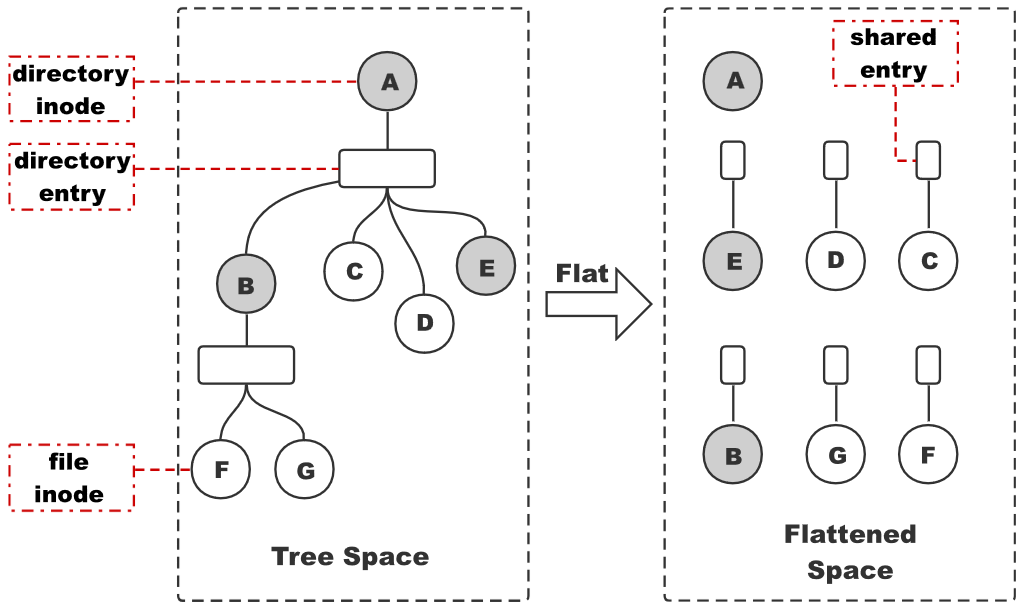
\includegraphics[scale=0.3]{flattened.png}
	\end{center}
	Fonte: [Dai et al., 2022]
\end{frame}

\subsubsection{Metadados de Valor Agregado}
\begin{frame}{Alto desempenho: (3) metadados de valor agregado}
	Em relação a \underline{metadados de valor agregado}:
	\begin{itemize}
		\item Feito sobre o gerenciamento padrão de metadados
		\item Aproveitar metadados para outras aplicações e consultas
		\item Registrar resultados intermediários que seriam descartados
		\item Informações de dependências entre arquivos
		\item ``Metadados ricos''
		\item Escalonador de \textit{workflow} pode se beneficiar
	\end{itemize}
\end{frame}

\subsection{Alta Disponibilidade}
\begin{frame}{Alta disponibilidade}
	A \textbf{alta disponibilidade} dos \textit{clusters} de MDS podem ser entendidas sob os seguintes olhares:
	\begin{enumerate}
		\item Baseada em cópia
		\item Baseada em \textit{log}
		\end{enumerate}
\end{frame}

\subsubsection{Baseada em cópia}
\begin{frame}{Alta disponibilidade: (1) baseada em cópia}
	O que é, prós e contras:
	\begin{itemize}
		\item Redundância
		\item Fazer cópia dos primários nos secundários
		\item Último ponto de salvamento
		\item Pode gerar inconsistências
		\item É possível adicionar técnicas de \textit{logs} para complementar
		\item Fazer troca em tempo-real
		\item Necessário consenso entre as partes
	\end{itemize}
\end{frame}

\begin{frame}{Alta disponibilidade: (1) baseada em cópia}
	\begin{center}
		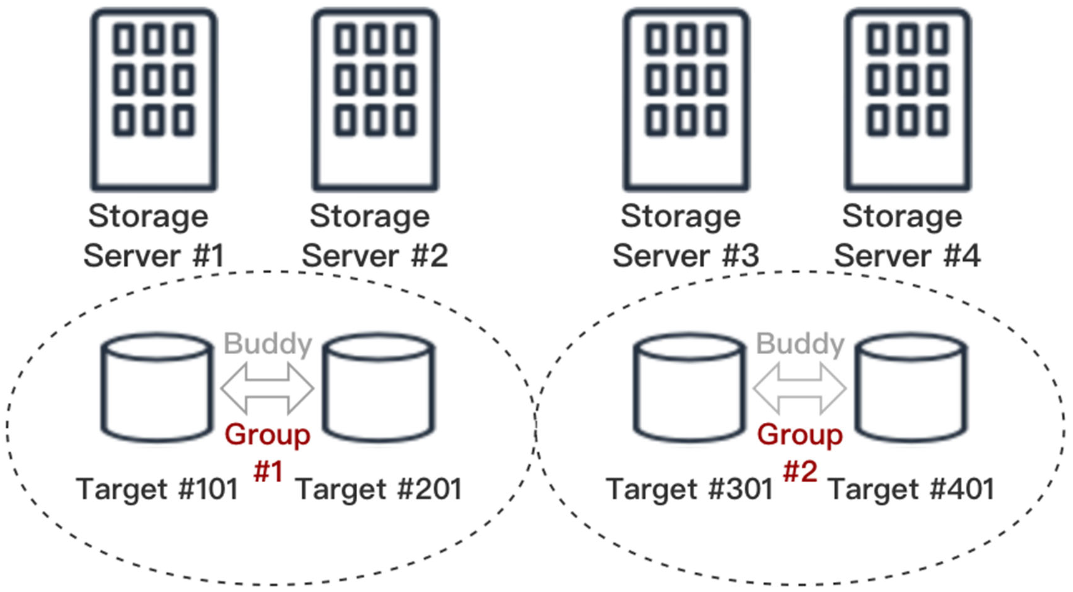
\includegraphics[scale=0.3]{ha-copia.png}
	\end{center}
	Fonte: [Dai et al., 2022]
\end{frame}

\subsubsection{Baseada em \textit{log}}
\begin{frame}{Alta disponibilidade: (2) baseada em \textit{log}}
	Para se evitar I/O, se usa \textit{cache}.
	
	Então \textit{logs} podem ser alternativa para não se perder essas informações.
	
	Sobre a disponibilidade baseada em \textit{log}:
	\begin{itemize}
		\item \textit{Logs} com travas/\textit{locks} distribuídos
		\item Em sistemas com discos compartilhados, pode levar a ``hot files''
		\item Em sistemas sem compartilhamentos (\textit{shared-nothing}), operações devem entrar nas transações
		\item Também deve haver consenso para se ter consistência
		\item Paxos ou Multi-Paxos são complexos e difíceis de implementar
		\item Raft tem sido usado
	\end{itemize}
\end{frame}

%\begin{frame}{}
%	T
%\end{frame}

%%%%%%%%%%%%%%%%%%%%%%%%%%%%%%%%%%%%%%%%%%%%%%%%%%%%%%%%%%%%%%%%%%%%%
\section{CEPH}
\subsection{Visão Geral}
\begin{frame}{Visão geral do CEPH}
	O sistema CEPH é:
	\begin{itemize}
		\item sistema de armazenamento distribuído
		\item código-fonte aberto
		\item Sage A. Weil. \textbf{Ceph: Reliable, Scalable, and High-Performance Distributed Storage}. PhD thesis, University of California, Santa Cruz, 2007.
		\item \url{https://docs.huihoo.com/ceph/Ceph-Reliable-Scalable-and-High-Performance-Distributed-Storage-2007.pdf}
		\item Suportado por Red Hat, Canonical, Intel
		\item Usado pelo CERN
		\begin{itemize}
			\item Large Hadron Collider (LHC)
			\item gera 25 PiB por ano
		\end{itemize}				
	\end{itemize}
\end{frame}

\subsection*{OFF-Topic}
\begin{frame}{OFF-Topic: LHC e buraco negro}
	\begin{center}
		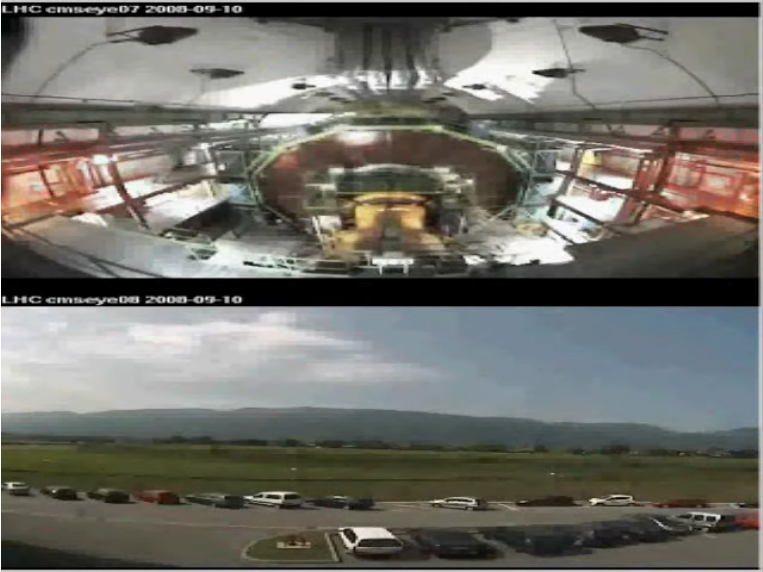
\includegraphics[scale=0.25]{buraco-negro-1.png}
	\end{center}
	Fonte: \url{https://www.youtube.com/watch?v=9JYkMhQ9gf8} \\
	\url{lhc-buraco-negro.mp4}
\end{frame}

\begin{frame}{OFF-Topic: LHC e buraco negro}
	Em 2008 ...
	\begin{block}{Para Hawking, projeto que 'recria Big Bang' não ameaça a Terra}
	O físico britânico Stephen Hawking afirma que não há perigo de que, ao ser acionado nesta quarta-feira, um gigantesco acelerador de partículas instalado numa área subterrânea da fronteira franco-suíça, possa criar um buraco negro capaz de engolir o planeta (e o resto do sistema solar) em questão de minutos - como temem alguns cientistas.
	\end{block}
	\url{https://www.bbc.com/portuguese/reporterbbc/story/2008/09/080909_lhc_hawking_mv}
\end{frame}

\begin{frame}{OFF-Topic: LHC e buraco negro}	
	Em 2013 ...
	\begin{block}{Algum dia o acelerador de partícula da CERN poderá criar um buraco negro?}
	Embora seja possível criar \underline{um ``micromini'' buraquinho negro} através do acelerador de partículas, nunca — jamais — a CERN poderá criar um buraco negro poderoso o suficiente para engolir a Terra. Segundo o site, \underline{o buraquinho seria tão pequenino} que seria difícil forçá-lo a engolir um único elétron.
	\end{block}
	
	\url{https://www.megacurioso.com.br/experiencias/36332-algum-dia-o-acelerador-de-particula-da-cern-podera-criar-um-buraco-negro-.htm}
\end{frame}

\begin{frame}{OFF-Topic: LHC e buraco negro}
	Em 2019 ...
	\begin{center}
		
\includegraphics[scale=0.2]{buraco-negro-2.jpg}
	\end{center}
	Fonte: \url{https://i.ytimg.com/vi/pw-56d2qfKM/maxresdefault.jpg}
	\newline
	
	\url{https://www.youtube.com/watch?v=pw-56d2qfKM}
\end{frame}

\begin{frame}{OFF-Topic: LHC e buraco negro}
	\begin{center}
		
\includegraphics[scale=0.25]{buraco-negro-3.jpg}
	\end{center}
	Fonte: \url{https://hypescience.com/wp-content/uploads/2019/04/meme-buraco-negro-publicidade-1.jpg}
\end{frame}

\subsection{Arquitetura}
\begin{frame}{Arquitetura do CEPH}
	\begin{center}
		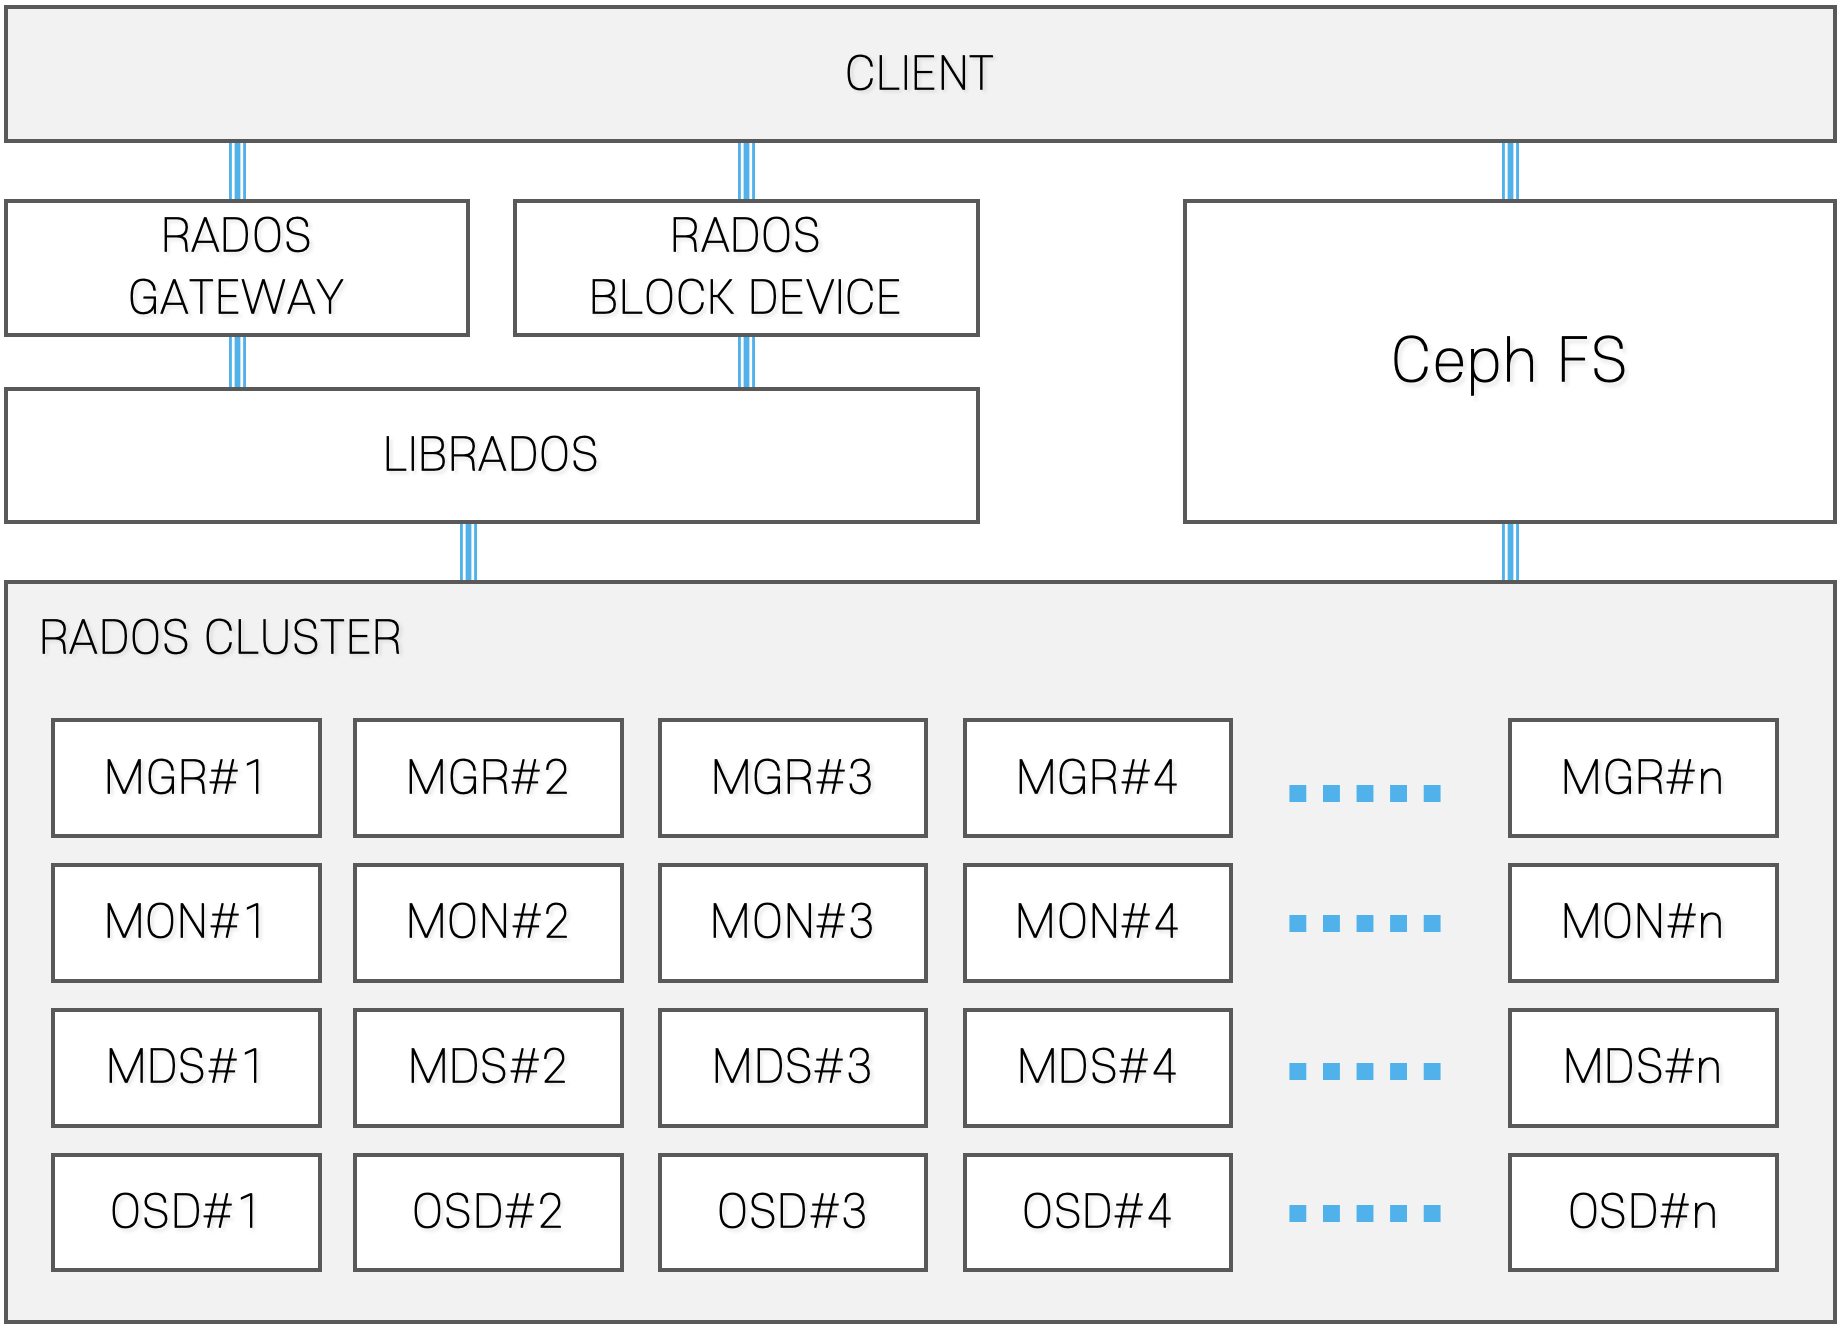
\includegraphics[scale=0.125]{ceph1.png}
	\end{center}
	Fonte: [Lee et al. 2021]
\end{frame}

\begin{frame}{Arquitetura do CEPH - Parte servidor}
	Fazem parte do \textit{Cluster} RADOS (\textit{Reliable Autonomous Distributed Object Storage}):
	\begin{description}
		\item[MGR] Gerenciador (\textit{Manager}). Monitora e orquestra sistema (exemplo, carga/\textit{load} e utilização de armazenamento), mesmo externo via painel web (\textit{dashboard}). Recomendados pelo menos 2; \pause
		\item[MON] Monitor. Mantém mapas dos recursos do cluster. Recomendado ter entre 3 e 7. \underline{Usa Multi-Paxos}; \pause
		\item[OSD] \textit{Daemon} de \textit{Object Storage Devices}. Acompanha o estado dos objetos, replicação, recuperação, rebalanceamento. Recomendado pelo menos 3; \pause
		\item[MDS] Servidor de metadados. Gerencia metadados do CephFS, se estiver presente na instância. Aceita comando como ls(1) e find(1).
	\end{description}
\end{frame}

\begin{frame}{Arquitetura do CEPH}
	\begin{center}
		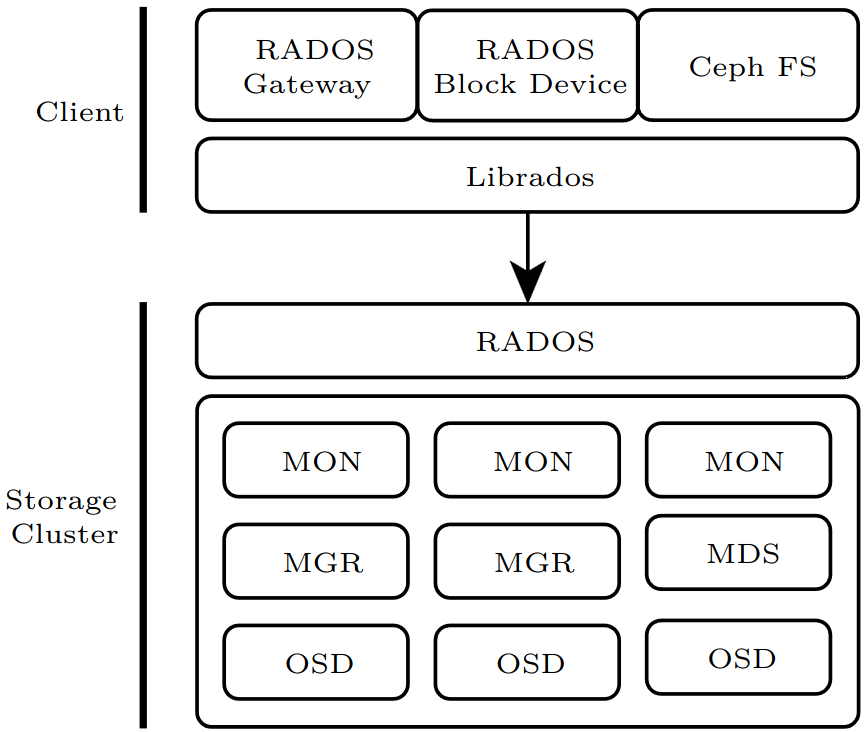
\includegraphics[scale=0.25]{ceph2.png}
	\end{center}
	Fonte: [Fernandes, 2021]
\end{frame}

\begin{frame}{Arquitetura do CEPH - Parte cliente}
	Parte cliente do sistema RADOS (\textit{Reliable Autonomous Distributed Object Storage}):
	\begin{description}
		\item[Librados] Biblioteca RADOS. Permite a comunicação com o \textit{Cluster} RADOS. Pode se comunicar diretamente com os OSD's; \pause
		\item[RBD] Dispositivo de Blocos de Dados (Rados Block Device). Provisiona dispositivos virtuais de blocos. Compatível com máquinas virtuais e Kubernates; \pause
		\item[RGW] Interface de armazenamento de objetos (Rados Gateway). Disponibiliza API para armazenar objetos e metadados. Compatível com Amazon S3 e OpenStack Swift; \pause
		\item[CephFS] Sistema de arquivos. Para armazenar dados. Usa o MDS. Compatível com POSIX: ls(1), find(1).
	\end{description}
\end{frame}

\subsection{Armazenamento}
\begin{frame}{Armazenamento de dados}
	\begin{center}
		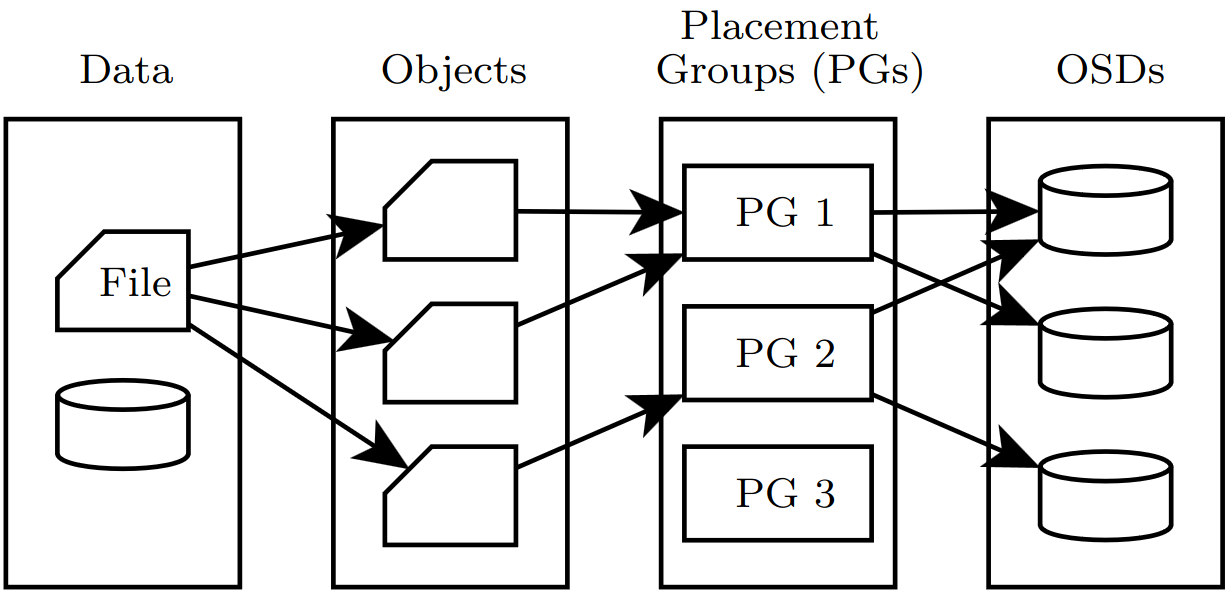
\includegraphics[scale=0.25]{ceph3.png}
	\end{center}
	Fonte: [Fernandes, 2021]
\end{frame}

\begin{frame}{Armazenamento de dados}
	O armazenamento de dados assim ocorre:
	\begin{enumerate}
		\item Os dados são divididos em objetos menores;
		\item Cada objeto é adicionado a um agrupamento (\textit{pool} de armazenamento) para compor um Grupo de Colocação (\textit{Placement Groups - PG}) disponível;
		\item Os PG são atribuídos a um OSD ...
		\begin{itemize}
			\item Sob supervisão do algoritmo CRUSH (\textit{Controlled Replication Under Scalable Hashing})
			\item Domínio de falhas
			\item Número de réplicas
			\item Estratégia de replicação
			\item Tipo de armazenamento (exemplo: HDD, SSD)
		\end{itemize}
	\end{enumerate}
\end{frame}

\subsection{Consenso}
\begin{frame}{Consenso no CEPH}
	O consenso no CEPH ocorre nos monitores (MON) e usa Multi-Paxos:
	\begin{center}
		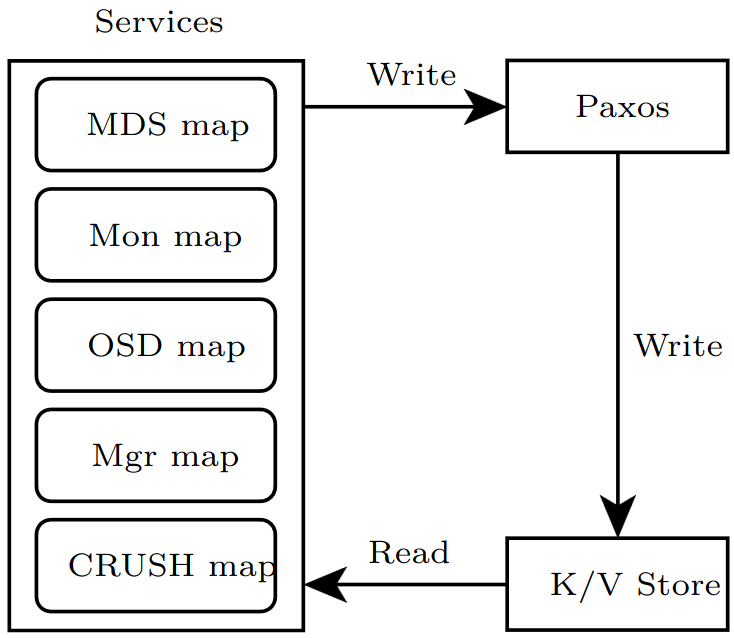
\includegraphics[scale=0.25]{ceph-paxos-1.png}
	\end{center}
	Fonte: [Fernandes, 2021]
\end{frame}

\begin{frame}{Consenso no CEPH}
	O consenso no CEPH ocorre nos monitores (MON) e usa Multi-Paxos:
	\begin{center}
		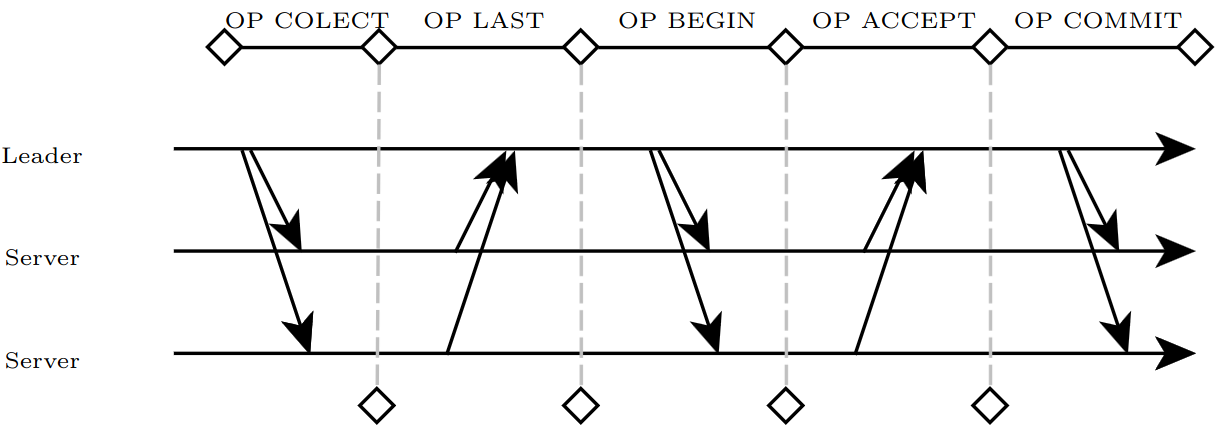
\includegraphics[scale=0.25]{ceph-paxos-2.png}
	\end{center}
	Fonte: [Fernandes, 2021]
\end{frame}

%%%%%%%%%%%%%%%%%%%%%%%%%%%%%%%%%%%%%%%%%%%%%%%%%%%%%%%%%%%%%%%%%%%%%
\section{Conclusão e trabalhos futuros}
\begin{frame}{Conclusão}
	Este trabalho apresentou ...
	\begin{itemize}
		\item uma introdução sobre sistemas de arquivos
		\item uma revisão sobre sistemas distribuídos
		\item um \textit{survey} sobre MDS
		\item o sistema CEPH
	\end{itemize}
\end{frame}

\begin{frame}{Trabalhos futuros}
	Meus trabalhos futuros:
	\begin{itemize}
		\item Realizar mais pesquisa sobre o estado da arte
		\item Acompanhar as defesas de TCC e de qualificação
		\item Fazer testes iniciais com o CEPH e o MDS
		\begin{itemize}
			\item MDS baseado em IA
			\item Novas mídias de armazenamento
			\item Serviços sem metadados
		\end{itemize}
	\end{itemize}
	
	\pause
	
	Trabalhos futuros desejáveis:
	\begin{itemize}
		\item Substituir o NFS por CEPH no DInf/UFPR
		\item Contribuir com a comunidade acadêmica
		\item Escrever artigos e TCCs, dissertações, teses
	\end{itemize}
\end{frame}

%%%%%%%%%%%%%%%%%%%%%%%%%%%%%%%%%%%%%%%%%%%%%%%%%%%%%%%%%%%%%%%%%%%%%
\section{Referências}
\begin{frame}{Referências}
    \begin{itemize}
    	\item Afonso das Neves Fernandes. \textbf{FORMAL VERIFICATION OF THE CEPH CONSENSUS ALGORITHM USING TLA$^{+}$}. Dissertação de mestrado, 2021. Universidade do Porto. URL: \url{https://repositorio-aberto.up.pt/bitstream/10216/139563/2/529181.pdf}
    	\item Lee, J.-Y., Kim, M.-H., Shah, S. A. R., Ahn, S.-U., Yoon, H., and Noh, S.-Y. (2021). \textbf{Performance evaluations of distributed file systems for scientific big data in fuse environment}. In Electronics 2021, 10, 1471, pages 1–16. Eletronics.
    	\item Dai, H; Wang, Y; Kent, K. B.; Zeng, L.; Xu, C. \textbf{The State of the Art of Metadata Managements in Large-Scale Distributed File Systems — Scalability, Performance and Availability}. IEEE TRANSACTIONS ON PARALLEL AND DISTRIBUTED SYSTEMS, 2022.
    \end{itemize}
\end{frame}

\begin{frame}[plain]{}
    \maketitle
\end{frame}

%%%%% Última página do modelo abaixo - PODE SER REMOVIDA, SE DESEJAR %%%%%
%{
%\usebackgroundtemplate%
%{%
%    
\includegraphics[width=\paperwidth,height=\paperheight]{ultima-pag-menor.jpg}%
%}
%\begin{frame}[plain]{}
%\end{frame}
%}
%%%%% Última página do modelo acima - PODE SER REMOVIDA, SE DESEJAR %%%%%
	
\end{document}